\documentclass[11pt]{article}
\usepackage[a4paper,landscape,margin=15mm]{geometry}
\usepackage{amsmath,amssymb,graphicx,booktabs,array,xcolor,hyperref,fancyhdr}
\definecolor{ink}{HTML}{183043}
\definecolor{violet}{HTML}{8749BA}
\definecolor{teal}{HTML}{008C83}
\hypersetup{pdftitle={Octagon surgery for the common C basis},colorlinks=true,urlcolor=teal,linkcolor=teal}
\pagestyle{fancy}\fancyhf{}\fancyhead[L]{\small\color{ink}Gr(4,16): surgery for the common $C$ basis}
\fancyhead[R]{\small Six individual promotion-orbit representatives}
\fancyfoot[L]{\footnotesize JSON-derived diagrams; exact boundary-fixed graph checks}
\fancyfoot[R]{\thepage}\setlength{\headheight}{14pt}
\setlength{\parindent}{0pt}\setlength{\parskip}{6pt}
\newcommand{\word}[1]{\texttt{#1}}
\newcommand{\heading}[1]{{\Large\bfseries\color{ink}#1}\par}
\newcommand{\fig}[1]{\par\begin{center}\includegraphics[width=.96\linewidth]{figures/#1.pdf}\end{center}\par}
\begin{document}
\heading{An octagon surgery explains all six correction diagrams}
\textbf{Finding.} In each of the six representatives, square moves expose an
alternating octagonal face with four hourglasses. A common cut-and-splice
operation on this face, followed by four bivalent contractions, produces exactly
the first correction diagram. In orbit 1 a second, ordinary-octagon unzip
produces the second correction. This gives a geometric analogue of the
benzene-chain picture, using an eight-sided configuration.

\textbf{Notation and the sign distinction.} Let $R_i$ denote the unsigned web
diagram reached by surgery, and let $W_i=W_{T_i}$. The earlier booklet's
representative pages give the following formulas, with $R_i$ abbreviating its
web invariant. In particular, orbits 2 and 5 have a plus sign.
\begin{center}\small
\begin{tabular}{clll}
\toprule
Individual orbit & $T_i$ (row word) & Correction diagram $R_i$ (row word) & Common-basis element\\
\midrule
1 & \word{1111222233334444} & \word{1121323142324344} & $C_1=W_1-R_1-Q$\\
2 & \word{1111222233343444} & \word{1121323142342344} & $C_2=W_2+R_2$\\
3 & \word{1111222323343444} & \word{1121323412342344} & $C_3=W_3-R_3$\\
4 & \word{1112122233343444} & \word{1123123142342344} & $C_4=W_4-R_4$\\
5 & \word{1112122323343444} & \word{1123123412342344} & $C_5=W_5+R_5$\\
6 & \word{1121223133424344} & \word{1231234123412344} & $C_6=W_6-R_6$\\
\bottomrule
\end{tabular}\end{center}
Here $Q=W_{\word{1212341234123434}}$. To use $C_i=W_i-P_i$ uniformly for
$i=2,\ldots,6$, set $P_2=-R_2$, $P_5=-R_5$, and $P_i=R_i$ otherwise.

\textbf{What has been checked.} The output diagrams agree with the specified
correction JSONs, fixing all sixteen boundary labels, vertex colors, edge
multiplicities, and cyclic orders. Both exposed-octagon presentations in each
complete square orbit give the same specified correction. No benzene face
occurs in any of the 176 presentations enumerated.

\textbf{Scope.} This is a verified \emph{geometric rule selecting correction
diagrams}. It is not a skein identity $W_i=R_i$, and does not derive the signs or
coefficients in the displayed $C_i$ formulas. Those are inherited from the
booklet, not proved by this surgery. Theta membership is not asserted.

\newpage
\heading{The local operation: splice across the ordinary sides}
\begin{minipage}[t]{.47\linewidth}
\vspace{0pt}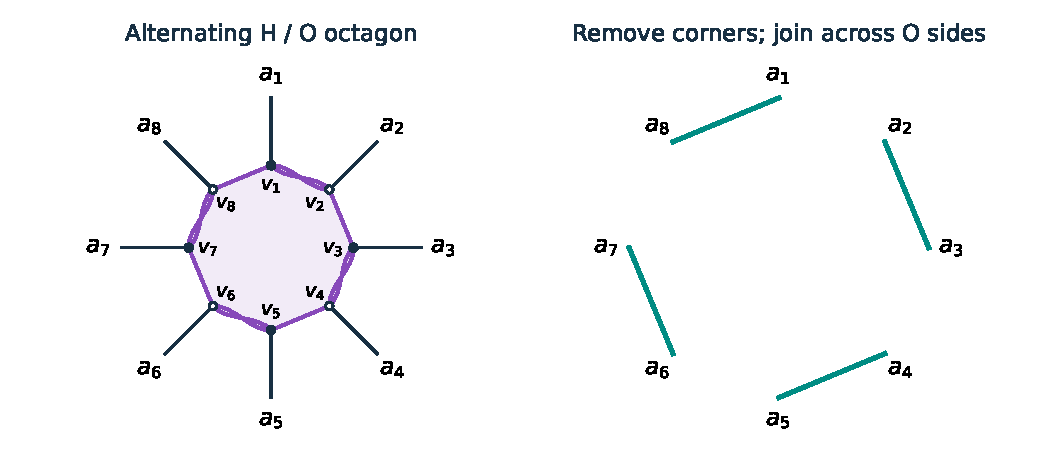
\includegraphics[width=\linewidth]{figures/local_rule.pdf}
\end{minipage}\hfill
\begin{minipage}[t]{.50\linewidth}
\vspace{0pt}
Write the exposed octagon cyclically as $v_1,\ldots,v_8$, with hourglass
sides $v_1v_2,v_3v_4,v_5v_6,v_7v_8$. Each corner has one exterior ordinary
edge $v_ja_j$. The ordinary sides are the other four sides.
\begin{enumerate}
\item Delete the eight corners and their incident edges.
\item Reconnect the exterior stubs across the ordinary sides:
\[
a_2a_3,\quad a_4a_5,\quad a_6a_7,\quad a_8a_1.
\]
\item In these six examples, each new edge duplicates an existing ordinary
edge. Replace each such pair by a multiplicity-2 \emph{hourglass}, retaining
the transported cyclic positions.
\item Contract the four resulting bivalent $2+2$ vertices, merging their
same-color neighbors. The result is $R_i$.
\end{enumerate}
\end{minipage}

\textbf{Normalization is part of the new operation.} Step 3 is a prescribed
replacement by an exterior-square edge with its hourglass twist. It is not an
assertion that two ordinary tensor strands equal an exterior-square strand
with coefficient one. The final bivalent contractions are the familiar
hourglass-web contraction moves; the whole splice is a new surgery, not an
existing invariant-preserving move.

Only the initial square moves preserve the invariant represented by the
diagram: $W_i=\widetilde W_i$ under the established square-move convention
\cite[Figures 2 and 9; Section 6.3]{GPPSS}. The surgery then changes the web to
$R_i$. In symbols, with different arrows for these different roles,
\[
W_i\ \overset{\text{square moves}}{=}\ \widetilde W_i
\quad\xrightarrow{\text{ordinary-side octagon surgery}}\quad R_i.
\]
The operation resembles benzene surgery by selecting alternating sides of an
even face, but here the face has eight sides and four hourglasses, not six
sides and three hourglasses.

\newpage
\heading{Individual orbit 2}
\textbf{Orbit 2.} $T_2=\word{1111222233343444}$, \quad
$R_2=W_{\word{1121323142342344}}$, \quad
$\boxed{C_2=W_2+R_2}$.
\fig{orbit_2}
The middle presentation is reached by five square moves. Splicing the four
ordinary octagon sides and making four $2+2$ contractions gives the right-hand
diagram. In the notation $C_2=W_2-P_2$, the signed correction is $P_2=-R_2$.

\newpage\heading{Individual orbit 3}
\textbf{Orbit 3.} $T_3=\word{1111222323343444}$, \quad
$R_3=W_{\word{1121323412342344}}$, \quad
$\boxed{C_3=W_3-R_3}$.
\fig{orbit_3}
Four square moves expose the same local octagon type. The identical surgery
gives $R_3$. The boundary labeling is unchanged throughout.

\newpage
\heading{Individual orbit 4}
\textbf{Orbit 4.} $T_4=\word{1112122233343444}$, \quad
$R_4=W_{\word{1123123142342344}}$, \quad
$\boxed{C_4=W_4-R_4}$.
\fig{orbit_4}
Five square moves expose the alternating octagon. After the same splice and
four contractions, the correction has eight internal vertices and two
hourglasses.

\newpage\heading{Individual orbit 5}
\textbf{Orbit 5.} $T_5=\word{1112122323343444}$, \quad
$R_5=W_{\word{1123123412342344}}$, \quad
$\boxed{C_5=W_5+R_5}$.
\fig{orbit_5}
Four square moves expose the octagon. The output has six internal vertices
and one hourglass. Again the geometry produces $R_5$, while the booklet's
signed correction is $P_5=-R_5$.

\newpage
\heading{Individual orbit 6: the correction becomes four stars}
\[
T_6=\word{1121223133424344},\qquad
R_6=W_{\word{1231234123412344}},\qquad
\boxed{C_6=W_6-R_6}.
\]
\fig{orbit_6}
Two square moves suffice. The exposed diagram has twenty internal vertices
and eight hourglasses; removing the octagon and performing the four bivalent
contractions leaves four internal vertices and no hourglasses.

The four star components have the following boundary blocks:
\[
\{1,2,3,16\},\quad \{4,5,6,7\},\quad
\{8,9,10,11\},\quad \{12,13,14,15\}.
\]
Consequently, as a product of Pl\"ucker coordinates, this correction is
proportional, with the orientation normalization determined by its source
JSON, to
\[
\Delta_{1,2,3,16}\,\Delta_{4,5,6,7}\,
\Delta_{8,9,10,11}\,\Delta_{12,13,14,15}.
\]
All four factors are cyclic interval Pl\"ucker coordinates. This identifies the
shape of the correction without using any theta-basis inference.

\textbf{A useful visual interpretation.} The surgery removes a central
alternating resonance region and leaves its exterior attachments to determine
the smaller web. Thus the correction need not arise from changing an isolated
benzene in the original drawing: it can be revealed only after square moves.

\newpage
\heading{Individual orbit 1: an octagon chain}
\[
\boxed{C_1=W_{\word{1111222233334444}}
-W_{\word{1121323142324344}}
-W_{\word{1212341234123434}}}
\]
\par\begin{center}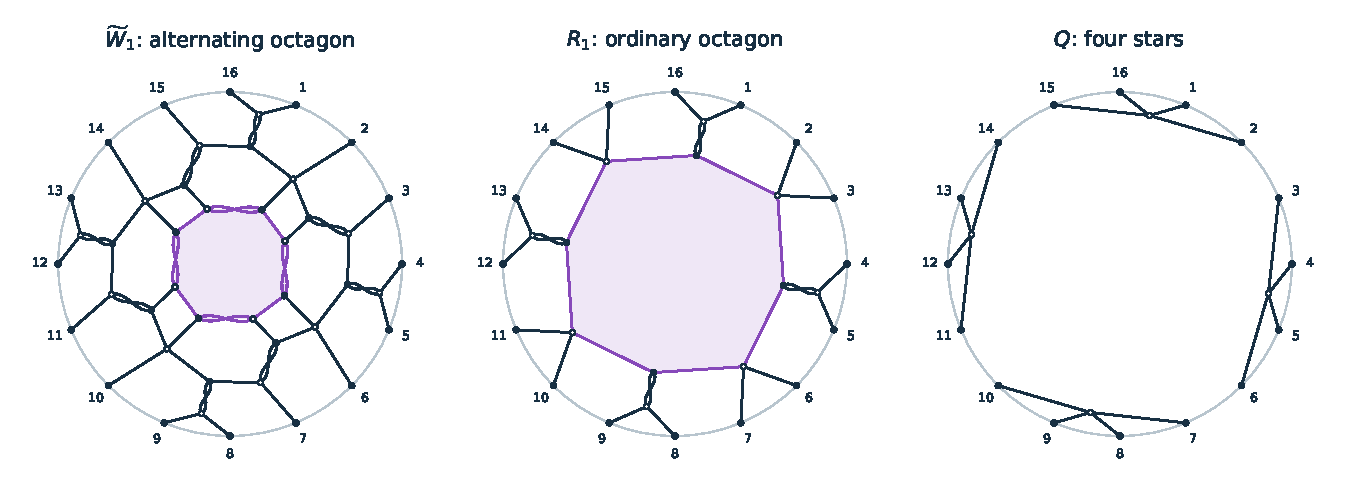
\includegraphics[width=.80\linewidth]{figures/chain.pdf}\end{center}\par
\textbf{First stage.} Five square moves expose the left-hand alternating
octagon. The ordinary-side splice and four contractions produce $R_1$, the
middle diagram. It has twelve internal vertices and four hourglasses.

\textbf{Second stage: unzip.} The middle diagram contains an ordinary
octagon. Alternating corners have either one exterior hourglass or two
exterior ordinary edges. Delete its eight vertices; split each exterior
hourglass into two ordinary attachments and connect them to the adjacent
ordinary stubs, one on each neighboring side of the face. Untwist the pair at
the surviving exterior endpoint. This last order convention is essential:
merely forgetting the twist gives a different ribbon graph.

More explicitly, write the octagon as $h_1,u_1,h_2,u_2,h_3,u_3,h_4,u_4$.
Let $h_i$ have its exterior hourglass to $z_i$. Let the exterior ordinary
stubs at $u_i$ lead to $a_i$ on the $h_i$ side and $b_i$ on the $h_{i+1}$
side. Replace the octagon and spokes by
\[
z_i a_i\quad\text{and}\quad z_i b_{i-1}\qquad(i\bmod 4),
\]
with the order at $z_i$ reversed relative to the removed hourglass pair.
The result is precisely $Q$, whose star blocks are
\[
\{1,2,15,16\},\quad\{3,4,5,6\},\quad
\{7,8,9,10\},\quad\{11,12,13,14\}.
\]
The geometric chain is $\widetilde W_1\rightsquigarrow R_1\rightsquigarrow Q$; $C_1$ subtracts both descendants.

\newpage
\heading{Verification, reproducibility, and the remaining algebraic question}
\begin{center}\small
\begin{tabular}{crrrrrr}
\toprule
Orbit & Square states & Exposing moves & Octagon presentations & Exposed internal/HG & Output internal/HG\\
\midrule
1 & 42 & 5 & 2 & 28 / 12 & 12 / 4\\
2 & 35 & 5 & 2 & 26 / 11 & 10 / 3\\
3 & 28 & 4 & 2 & 24 / 10 & 8 / 2\\
4 & 30 & 5 & 2 & 24 / 10 & 8 / 2\\
5 & 23 & 4 & 2 & 22 / 9 & 6 / 1\\
6 & 18 & 2 & 2 & 20 / 8 & 4 / 0\\
\bottomrule
\end{tabular}\end{center}
\textbf{Exact checks.} Breadth-first search enumerated each complete square
orbit, checking the three trip permutations after every move. For every
exposed alternating octagon, the splice produces four doubled pairs and four
bivalent $2+2$ contractions. A boundary-fixed isomorphism to the correction
JSON preserves colors, multiplicities and all compressed cyclic orders, with
each multiplicity-2 edge understood as the standard hourglass. All twelve
checks pass. The second-stage unzip also matches $Q$ with these data. These
checks are combinatorial and independent of the drawing layout.

\textbf{Files.} The source bundle contains the LaTeX, vector illustrations,
original graph JSONs, generated JSONs for exposed/spliced/contracted diagrams,
the complete matching certificates, square-move paths, and replay code.
The generated schema stores \texttt{rotation\_ccw} as a cyclic list of
neighbors; multiplicity-2 neighbors occur once in this compressed list.
Original JSONs retain their full strand data. Figure coordinates are for
display only; topology is taken from the stored rotation systems.

\textbf{What remains to prove.} To promote this geometric explanation to an
algebraic construction of the common basis, one must derive the signed
coefficients from the FLL pairing or from an appropriate local relation. A
general surgery rule would also need a proof of compatibility with arbitrary
square-move presentations. The present finite check establishes consistency
on these six entire square orbits, not on all webs in $\operatorname{Gr}(4,16)$.

\begin{thebibliography}{9}\small
\bibitem{GPPSS} C. Gaetz, O. Pechenik, S. Pfannerer, J. Striker, and J. P.
Swanson, \emph{Rotation-invariant web bases from hourglass plabic graphs},
\href{https://arxiv.org/abs/2306.12501}{arXiv:2306.12501}.
Figures 2 and 9 and Section 6.3 supply the square-move and contraction context;
the octagon correction surgeries here are computational observations.
\bibitem{booklet} \emph{Common\_C\_basis\_68\_cases\_and\_theta\_tests.pdf},
individual orbit representative pages 5--10. Source of the six common-basis
formulas and their sign conventions.
\bibitem{data} Z. Saron, \emph{Tableaux--Hourglass Plabic Graphs and Web Duality},
\href{https://github.com/zsaron-555/Tableaux-Hourglass-Plabic-Graphs-and-Web-Duality}{project repository}.
The supplied graph JSONs and the earlier booklet, rather than a new pairing
calculation, are the inputs to this comparison.
\end{thebibliography}
\end{document}
